% Python 文件读写

\pentry{Python 入门\upref{Python}}

学习处理文件和保存数据可让你的程序使用起来更容易: 用户将能够选择输入什么样的数据, 以及在什么时候输入; 用户使用你的程序做一些工作后, 可将程序关闭, 以后再接着往下做.
\subsection{Python文件读写的方法}
\textbf{open() 方法}

Python \verb|open()| 方法用于打开一个文件,并返回\textbf{文件对象(file object)},在对文件进行处理过程都需要使用到这个函数,如果该文件无法被打开,会抛出错误.

\verb|open()| 函数常用形式是接收两个参数:\textbf{文件名(file)}和\textbf{模式(mode)}.
\begin{lstlisting}[language=python]
open(file, mode='r')
\end{lstlisting}
此方法有很多其他参数,一般情况下用不到.其中\verb|file| 必需,是文件路径(相对或者绝对路径); \verb|mode| 可选,代表文件打开模式.打开模式有多种方式.
\begin{table}[ht]
\centering
\caption{打开模式}\label{PyFile_tab1}
\begin{tabular}{|c|c|}
\hline
r & 以只读方式打开文件 \\
\hline
w & 打开一个文件只用于写入.如果该文件已存在则打开文件,并从开头开始编辑,即原有内容会被删除.如果该文件不存在,创建新文件. \\
\hline
b & 二进制模式 \\
\hline
+ & 打开一个文件进行更新(可读可写) \\
\hline
a & 打开一个文件用于追加.如果该文件已存在, 新的内容将会被写入到已有内容之后; 如果该文件不存在, 创建新文件进行写入 \\
\hline
&上述方式组合使用   \\
\hline
\end{tabular}
\end{table}

使用 \verb|open()| 方法一定要保证关闭文件对象,即调用 \verb|close()| 方法. 例如计算机上有一个文件名为\verb|file.txt|的文件, 内容如\autoref{PyFile_fig2}所示, 需要读取并输出. 代码如下
\begin{figure}\label{PyFile_fig2}[ht]
\centering
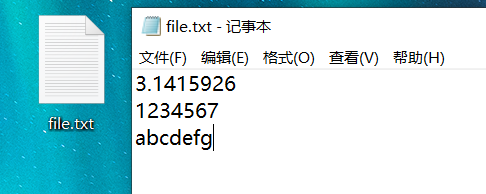
\includegraphics[width=5cm]{./figures/PyFile_1.png}
\caption{file文件内容} \label{PyFile_fig1}
\end{figure}
\begin{lstlisting}[language=matlab]
fo=open(r'C:\Users\shizy\Desktop\file.txt')
print("文件名: ", fo.name)
print("是否已关闭 : ", fo.closed)
print("访问模式 : ", fo.mode)
str = fo.read()
print(str)
fo.close()
\end{lstlisting}
输出如下
\begin{lstlisting}[language=python]
文件名:  C:\Users\shizy\Desktop\file.txt
是否已关闭 :  False
访问模式 :  r
3.1415926
1234567
abcdefg
\end{lstlisting}
上述代码第一个\verb|open|方法前面我们添加了一个\verb|r|, 表示原生字符串, 否则\verb|\|会对字符串进行转义处理. 当然也可以不加\verb|r|, 而使用两个\verb|\|, 效果一样. 我们在程序2-4行分别使用了文件的三种其他方法:

\verb|file.closed| 返回 true 如果文件已被关闭,否则返回 false.

\verb|file.mode| 返回被打开文件的访问模式.

\verb|file.name| 返回文件的名称.


\textbf{write() 方法}

\verb|write()|方法可将任何字符串写入一个打开的文件.需要重点注意的是,Python字符串可以是二进制数据,而不是仅仅是文字.\verb|write()|方法不会在字符串的结尾添加换行符 \verb|\n|. 语法如下:
\begin{lstlisting}[language=python]
fo = open("file2.txt", "wb")
fo.write( "Hello Python\n");
# 关闭打开的文件
fo.close()
\end{lstlisting}

\textbf{readline() 方法}

\verb|readline()| 会从文件中读取单独的\textbf{一行}.换行符为 '\verb|\n|'.\verb|readline()| 如果返回一个空字符串, 说明已经已经读取到最后一行.

\textbf{readlines() 方法}

\verb|readlines()| 将以列表的形式返回该文件中包含的\textbf{所有行},列表中的一项表示文件的一行.如果设置可选参数 \verb|sizehint|, 则读取指定长度的字节, 并且将这些字节按行分割.

上面介绍的文件读写方法虽然没问题,但是一般情况下我们不使用,而是使用\verb|with| 方法.从而避免忘记关闭文件导致的不可预料的结果.


\subsection{从文件中读取数据}
\subsubsection{读取整个文件}
下面的程序打开并读取这个文件, 再将其内容显示到屏幕上:
\begin{lstlisting}[language=python]
with open('file.txt') as f:
contents = f.read()
print(contents)
\end{lstlisting}
在这个程序中, 关键字\verb|with| 在不再需要访问文件后将其关闭. 在这个程序中, 注意到我们调用了\verb|open()|, 但没有调用\verb|close()|; 你也可以调用\verb|open()| 和\verb|close()| 来打开和关闭文件, 但这样做时, 如果程序存在错误, 导致\verb|close()| 语句未执行, 文件将不会关闭. 这看似微不足道, 但未妥善地关闭文件可能会导致数据丢失或受损. 如果在程序中过早地调用\verb|close()|, 你会发现需要使用文件时它已关闭, 无法访问, 这会导致更多的错误. 并非在任何情况下都能轻松确定关闭文件的恰当时机, 但通过使用前面所示的结构, 可让Python去确定: 你只管打开文件, 并在需要时使用它, Python自会在合适的时候自动将其关闭.

\subsubsection{逐行读取}
读取文件时, 常常需要检查其中的每一行: 你可能要在文件中查找特定的信息, 或者要以某种方式修改文件中的文本.
\begin{lstlisting}[language=python]
with open('file.txt') as f:
    for line in f:
        print(line)
\end{lstlisting}

利用\verb|with|来对文件的操作与上一节类似,这里不再赘述.

\subsection{数据存储}
很多程序都要求用户输入某种信息. 不管专注的是什么, 程序都把用户提供的信息存储在列表和字典等数据结构中.  用户关闭程序时, 你几乎总是要保存他们提供的信息; 一种简单的方式是使用模块\verb|json| 来存储数据.

模块\verb|json| 让你能够将简单的Python数据结构转储到文件中, 并在程序再次运行时加载该文件中的数据. 你还可以使用\verb|json| 在Python程序之间分享数据. 更重要的是, \verb|json|数据格式并非Python专用的, 这让你能够将以\verb|json|格式存储的数据与使用其他编程语言的人分享. 这是一种轻便格式, 很有用, 也易于学习.

\subsubsection{使用json.dump() 和json.load()}
我们来编写一个存储一组数字的简短程序, 再编写一个将这些数字读取到内存中的程序. 第一个程序将使用\verb|json.dump()| 来存储这组数字, 而第二个程序将使
用\verb|json.load()|.

函数\verb|json.dump()| 接受两个实参: 要存储的数据以及可用于存储数据的文件对象. 下面演示了如何使用\verb|json.dump()| 来存储数字列表.
\begin{lstlisting}[language=python]
import json
numbers = [2, 3, 5, 7, 11, 13]
filename = 'numbers.json'
with open(filename, 'w') as f_obj:
    json.dump(numbers, f_obj)
\end{lstlisting}
我们先导入模块\verb|json|, 再创建一个数字列表. 在第三行处, 我们指定了要将该数字列表存储到其中的文件的名称. 通常使用文件扩展名\verb|.json|来指出文件存储的数据为\verb|json|格式. 接下来, 我们以写入模式打开这个文件, 让\verb|json| 能够将数据写入其中. 在第五行处, 我们使用函数\verb|json.dump()| 将数字列表存储到文件\verb|numbers.json|中.

下面再编写一个程序, 使用\verb|json.load()| 将这个列表读取到内存中:

\begin{lstlisting}[language=python]
import json
filename = 'numbers.json'
with open(filename) as f_obj:
   numbers = json.load(f_obj)
print(numbers)
\end{lstlisting}
